\Mysection{Introduction}

\STANDARD{Project Scope}
{
    This project focuses on forecasting Germany's inflation using the Consumer Price Index (CPI) as a time series.

    \vspace{0.2cm}
    \begin{itemize}
        \item The main objective is to predict future CPI values from historical monthly observations.
        \item The analysis focuses on patterns such as trend, seasonality, and autocorrelation.
        \item Classical forecasting models, ARIMA, ETS, and SARIMA, are compared to assess how well they capture inflation dynamics.
    \end{itemize}
}


\Mysection{Motivation}

\STANDARD{Motivation}
{
    \begin{itemize}
        \item CPI measures the average change in prices of a typical basket of goods and services over time.
        \item CPI is one of the main indicators used to track inflation in Germany.
        \item Forecasting CPI helps us understand how inflation may develop in the near future.
        \item This is useful for economic analysis, planning, and comparing changes over time.
        \item The project also shows how time series models can turn past inflation data into interpretable forecasts.
    \end{itemize}

    {\scriptsize For more on the basket of goods, see: \url{https://www.destatis.de/EN/Themes/Economy/Prices/Consumer-Price-Index/BasketGoodsWeightingPattern.html}}
}

\STANDARD{Objectives}
{
    \begin{itemize}
        \item Forecast future CPI values from historical monthly observations.
        \begin{itemize}
            \item Prepare the CPI data so it is stable over time and suitable for forecasting models.
            \item Identify and interpret long-term trend and possible seasonal effects.
        \end{itemize}
        \item Compare and evaluate models and indentify which best captures Germany's CPI dynamics.
    \end{itemize}

}

\Mysection{Methodology}

\STANDARD{KDD-Based Workflow}
{
    \centering
    % === Diagram style definitions ===
    % mainblock  = default workflow block
    % dbblock    = database/source block
    % mineblock  = data mining block
    % modelblock = deployment blocks (new data / inference / results)
    % evalblock  = evaluation block
    % flow       = solid arrow
    % lineflow   = plain line used in feedback path routing
    \tikzstyle{mainblock} = [rectangle, rounded corners=2pt, minimum width=2.55cm, minimum height=1.15cm, text centered, align=center, draw=HSELblau, fill=blue!18]
    \tikzstyle{dbblock} = [mainblock, fill=red!18]
    \tikzstyle{mineblock} = [mainblock, fill=green!22]
    \tikzstyle{modelblock} = [mainblock, fill=yellow!22]
    \tikzstyle{evalblock} = [mainblock, minimum width=3.0cm, minimum height=1.05cm, fill=blue!18]
    \tikzstyle{flow} = [->, >=stealth, draw=HSELblau]
    \tikzstyle{lineflow} = [-, >=stealth, draw=HSELblau]
    \begin{tikzpicture}[scale=0.53, every node/.style={transform shape}]
        % ==============================================================
        % OUTER FRAMES
        % Syntax: (left,bottom) rectangle (right,top)
        % - increase horizontal length -> increase right x OR decrease left x
        % - reduce horizontal length    -> decrease right x OR increase left x
        % - increase downward depth     -> decrease bottom y
        % - reduce downward depth       -> increase bottom y
        % - increase upward height      -> increase top y
        % ==============================================================
        % Deployment outer frame
        \draw[draw=HSELblau, line width=0.5pt] (-1.8,1.3) rectangle (18.3,5.0);
        % Development outer frame
        \draw[draw=HSELblau, line width=0.5pt] (-1.8,-3.8) rectangle (18.3,1.0);

        % Monitoring highlight area inside the deployment frame
        % Same rectangle rules as above. Lower the first y-value to make it taller downward.
        \fill[HSELhellblau!35] (6.0,2.0) rectangle (17.8,4.55);
        \draw[draw=HSELblau, line width=0.5pt] (6.0,2.0) rectangle (17.8,4.55);

        % Monitoring title position: (x,y) = (left/right, down/up)
        \node[font=\small\bfseries, text=HSELblau] at (12.0,4.15) {Monitoring};

        % ==============================================================
        % TOP / DEPLOYMENT BLOCKS
        % Move blocks horizontally by changing x.
        % Move blocks vertically by changing y.
        % Keep inference x = mining x for a straight vertical connector.
        % ==============================================================
        \node (db) [dbblock] at (0,3.25) {Database\\(Destatis CPI)};
        \node (newdata) [modelblock] at (8.0,3.25) {New Data};
        \node (inference) [modelblock] at (12.0,3.25) {Model,\\Inference};
        \node (results) [modelblock] at (16.0,3.25) {Results};

        % Bottom / development workflow blocks
        \node (sel) [mainblock] at (0,0) {Data\\Selection};
        \node (prep) [mainblock] at (4.0,0) {Data\\Preprocessing};
        \node (trans) [mainblock] at (8.0,0) {Data\\Transformation};
        \node (mine) [mineblock] at (12.0,0) {Data\\Mining};
        \node (eval) [evalblock] at (12.0,-2.65) {Evaluation \&\\Verification};

        % Frame labels
        % Change x to recenter horizontally, y to move label up/down.
        \node[font=\small\bfseries] at (-0.7,-3.5) {Development};
        \node[font=\small\bfseries] at (-0.7,4.70) {Deployment};

        % ==============================================================
        % MAIN SOLID FLOW ARROWS
        % If a line is slanted, align the relevant node x/y positions.
        % ==============================================================
        \draw [flow] (db.south) -- (sel.north);
        \draw [flow] (sel.east) -- (prep.west);
        \draw [flow] (prep.east) -- (trans.west);
        \draw [flow] (trans.east) -- (mine.west);

        \draw [flow] (mine.north) -- (inference.south);
        \draw [flow] (newdata.east) -- (inference.west);
        \draw [flow] (inference.east) -- (results.west);

        \draw [flow] (mine.south) -- (eval.north);
        \draw [lineflow] (eval.west) -- (0.0,-2.65);
        \draw [flow] (0.0,-2.65) -- (sel.south);
        \draw [flow] (4.0,-2.65) -- (4.0,-1.05) -- (prep.south);
        \draw [flow] (8.0,-2.65) -- (8.0,-1.05) -- (trans.south);

        % Dashed feedback / monitoring-related paths
        % results -> eval = deployment results feed back into evaluation
        % newdata -> db    = refreshed data loop / data arrival path
        \draw [flow, dashed, red] (results.south) -- (16.0,-2.65) -- (eval.east);
        \draw [flow, dashed, red] (newdata.west) -- (1.30,3.25) -- (db.east);
        % \draw [flow, dashed, red] (db.east) -- (1.25,3.25) -- (newdata.west) ;
    \end{tikzpicture}

    \vspace{0.25cm}
    \begin{itemize}
        \item The lower part shows the core KDD development workflow from data selection to evaluation, while the upper part extends it into deployment through monitoring, new incoming data, model inference, results, and feedback loops for future updates.
    \end{itemize}
}

\Mysection{Dataset}
\STANDARD{Dataset}
{
            \begin{itemize}
                \item Source: Destatis GENESIS database, table 61111-0002.
                \item Link: \url{https://www-genesis.destatis.de/datenbank/online/statistic/61111/table/61111-0002}
                \item Monthly CPI observations for Germany from 1991 to 2026.
                \item Core fields: Date and CPI.
                \item With 2020 = 100, values below 100 mean lower prices than in 2020.
                \item Suitable for classical forecasting because the series is chronological and evenly spaced.
            \end{itemize}
}

\STANDARD{Dataset}
{
    \begin{center}
        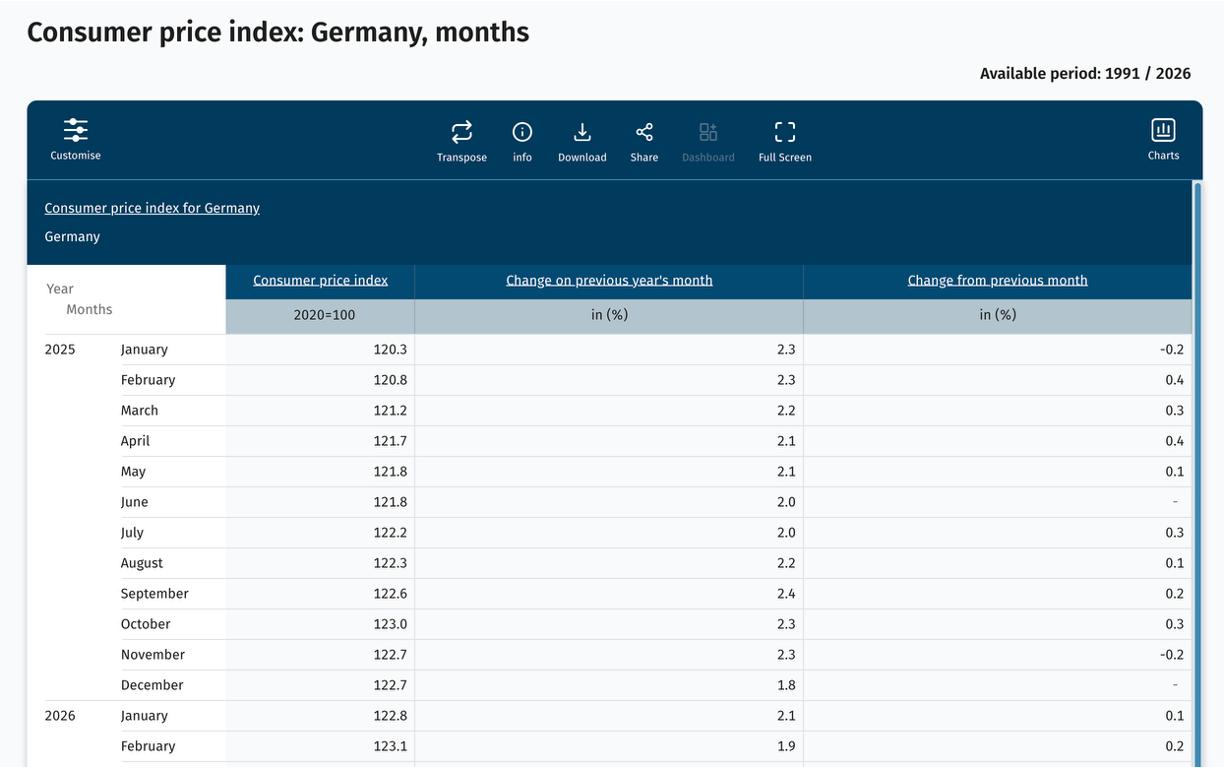
\includegraphics[width=0.9\textwidth]{img/dataset.png}

        \vspace{0.2cm}
        {\scriptsize Figure: Preview of the Germany CPI dataset. Source: \url{https://www-genesis.destatis.de/datenbank/online/statistic/61111/table/61111-0002}}
    \end{center}
}


\Mysection{Data Transformation}
\STANDARD{Data Transformation}
{
    \begin{itemize}
        \item We break the CPI data into trend, seasonality, and random variation.
        \item We use the ADF test to check whether the data is stable over time.
        \item If the data is not stable, differencing is used by comparing each value with the previous one.
        \item ACF and PACF plots help us see how current values relate to past values.
        \item The goal is to prepare the data so forecasting models can work better.
    \end{itemize}
}

\Mysection{Data Mining}
\STANDARD{Data Mining}
{
    \begin{itemize}
        \item In this phase, we train forecasting models on the prepared CPI data.
        \item ARIMA uses past values and past errors to make forecasts.
        \item ETS models the level, trend, and seasonality of the series directly.
        \item SARIMA is similar to ARIMA, but also includes seasonal patterns.
        \item The goal is to compare which model forecasts future CPI values best.
    \end{itemize}
}

\Mysection{Evaluation}
\STANDARD{Evaluation}
{
    Since the objective is forecasting continuous values, regression-based metrics are used.
    \vspace{0.25cm}
    \begin{itemize}
        \item RMSE captures overall prediction error and penalizes large deviations.
        \item MAE provides a stable and interpretable average error.
        \item MAPE allows comparison in percentage terms, making results easier to interpret.
    \end{itemize}

    \begin{center}
        \footnotesize
        \begin{tabular}{|p{1.0cm}|p{3.5cm}|p{4.5cm}|}
            \hline
            \textbf{Metric} & \textbf{Full Form} & \textbf{Description} \\
            \hline
            RMSE & Root Mean Squared Error & Penalizes larger errors more heavily \\
            \hline
            MAE & Mean Absolute Error & Average absolute difference between actual and predicted values \\
            \hline
            MAPE & Mean Absolute Percentage Error & Expresses error as a percentage \\
            \hline
        \end{tabular}
    \end{center}


}


\Mysection{Expected Output}
\STANDARD{Expected Output}
{
    \begin{itemize}
        \item A ranked comparison of ARIMA, ETS, and SARIMA on German CPI forecasting.
        \item Interpretable findings on trend, seasonality, and model suitability.
        \item A reproducible workflow that can be updated as new CPI data becomes available.
    \end{itemize}

    \vspace{0.2cm}
    \begin{center}
        \footnotesize
        \begin{tabular}{|l|c|c|c|}
            \hline
            \textbf{Model} & \textbf{RMSE} & \textbf{MAE} & \textbf{MAPE} \\
            \hline
            ARIMA & TBD & TBD & TBD \\
            \hline
            ETS & TBD & TBD & TBD \\
            \hline
            SARIMA & TBD & TBD & TBD \\
            \hline
        \end{tabular}
    \end{center}
}

\Mysection{Potential Delighters}

\STANDARD{Potential Delighters}
{
    \begin{itemize}
        \item Add forecast confidence intervals to quantify uncertainty.
        {\scriptsize
        \begin{itemize}
            \setlength{\itemsep}{0.10em}
            \item Compute prediction intervals, Eg. 80\% and 95\% for all models.
            \item Visualize upper and lower bounds together with the forecasts.
            \item Compare confidence intervals across ARIMA, ETS, and SARIMA.
        \end{itemize}
        }
        \vspace{10pt}
        \item Investigate structural breaks or inflation shocks in the CPI series.
        {\scriptsize
        \begin{itemize}
            \setlength{\itemsep}{0.10em}
            \item Identify periods of sudden change, such as COVID-19/energy crisis.
            \item Analyze deviations from the long-term inflation trend.
            \item Observe model performance before and after structural breaks.
            \item Interpret possible economic reasons behind these shocks.
        \end{itemize}
        }

    \end{itemize}
}

\STANDARD{Keyword Full Forms}
{
    \begin{itemize}
        \item CPI: Consumer Price Index
        \item ADF: Augmented Dickey-Fuller
        \item Stationarity: a stable time-series property
        \item ACF: Autocorrelation Function
        \item PACF: Partial Autocorrelation Function
        \item ETS: Error, Trend, Seasonality
        \item ARIMA: AutoRegressive Integrated Moving Average
        \item SARIMA: Seasonal AutoRegressive Integrated Moving Average
    \end{itemize}
}

\STANDARD{Keyword Definitions}
{
    \begin{itemize}
        \item CPI: the inflation indicator being forecast in this project.
        \item ADF: statistical test used to check whether the time series is stationary.
        \item Stationarity: stable statistical behavior over time, required by ARIMA-type models.
        \item Decomposition: separation of the time series into trend, seasonal, and residual components.
        \item Differencing: transformation that subtracts previous values to remove trend and improve stationarity.
        \item ACF: diagnostic tool for temporal correlation across lags.
        \item PACF: diagnostic tool that helps identify direct lag relationships and model order.
        \item ETS, ARIMA, SARIMA: the three forecasting model families compared in the project.
    \end{itemize}
}
